\subsection *{Omán - země sultána, nafty za 10 korun a pánských pyžam}
\label{sub:omán_-_země sultána_ nafty_za_10_korun_a_pánských_pyžam}

V rámci svého studia na Fildě jsem se vydal na kurz arabštiny do Ománu. Fakulta mi tak umožnila strávit 2 měsíce na Univerzitě Sultána Qábúse pro výuku arabštiny v Manahu – malé vesnici na pomezí Zelených hor a pouště. Studium na Univerzitě zní honosně, ale v Manahu je fakulta specializovaná pouze na výuku arabštiny pro studenty, jejichž rodným jazykem není arabština a tím pádem to je spíše komorní záležitost. Dohromady se nás sešlo 25 nadšenců různých věků a velikostí z celého světa – od Indonésie až po Velkou Británii. 

Nevím, co se vám vybaví, když se řekne Omán. Já každopádně před odletem myslel na vedro, velbloudy a mrakodrapy. Na konci října bylo v Praze okolo 0, Maskat (hlavní město) mě přivítal ve 2 v noci svěžími 30 stupni. Velbloudy tu vídám celkem pravidelně – kus od koleje je velbloudí farma (plot s beduínem a velbloudy) – a mrakodrapy tu nejsou, protože je SQ(sultán Qábús) zakázal – rušily by urbanistický ráz města! 

Jinak ale tato zem, původně zvaná Magan, působí úplně jinak, než jiné arabské státy.

\begin{center}
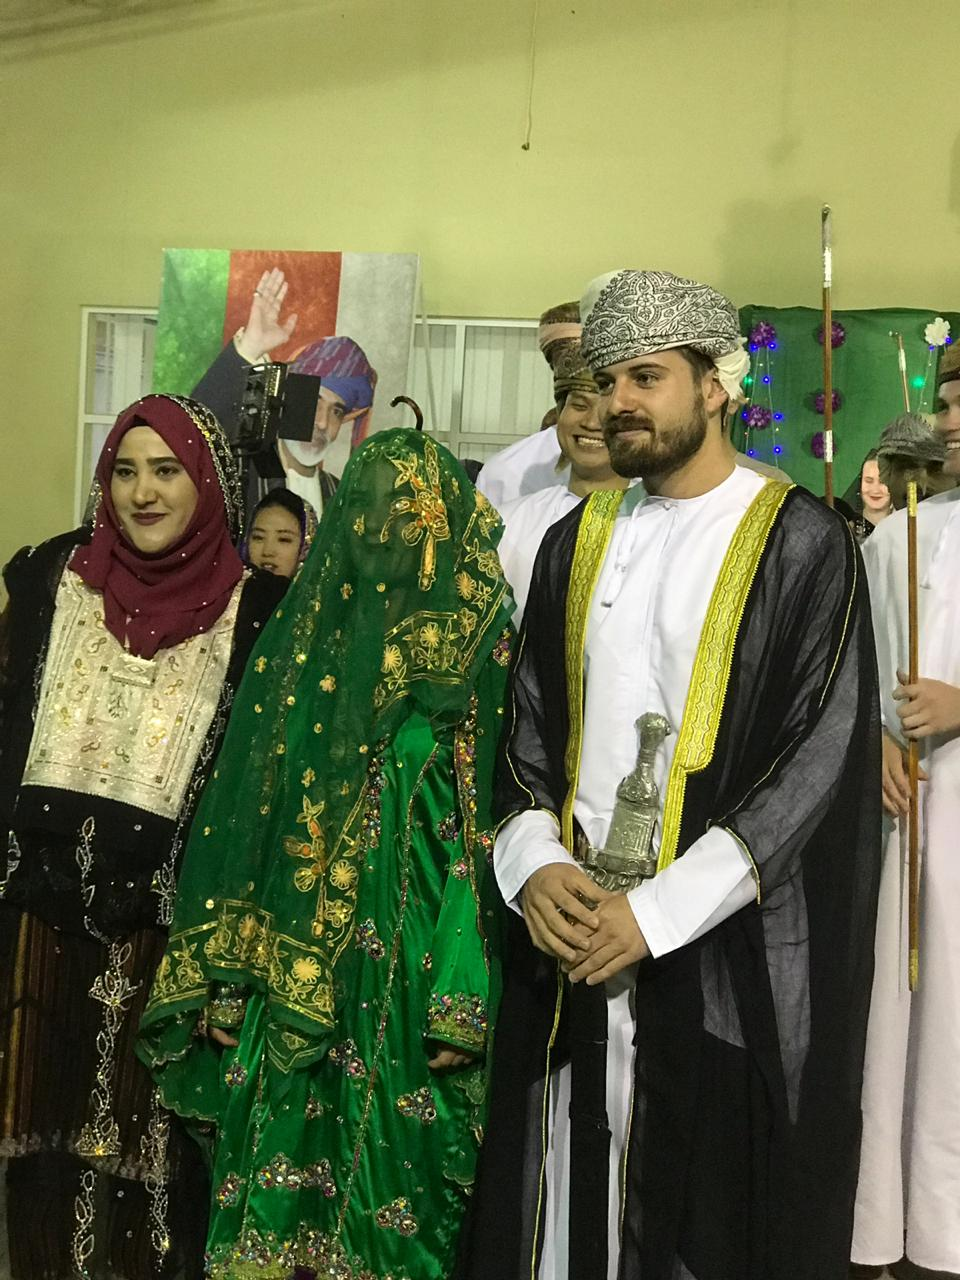
\includegraphics[width=8cm]{img/udo_clanky/Humr_oman.jpg}
\end{center}

Za prvé, všude jsou fotky SQ v různých pózách (sultán Qábús sedící, klečící, mávající, vzdávající se, usmívající se, važný, s holí a s mečem) a vše se tady jmenuje po SQ  - nemocnice, univerzity, školky, mešity, knihovny, lékárny, městské čtvrti - dokonce i na všech bankovkách je jen sultán. Oproti šíleným diktátorům a generálům jinde mají Ománci svého sultána rádi a neustále se usmívají… Také se k tomu váží příjemně časté oslavy narozenin Sultána, státních svátků, narozenin proroka, arabštiny a dalších příležitostných možností k tomu udělat si volno.

Za druhé, díky masivní výstavbě dálnic to tu vypadá jako v USA, akorát místo lánů kukuřice je kamenitá poušť a hory. Jako v USA to tu i funguje – bez auta a klimatizace se daleko nedostanete. Ve škole svádíme neustálý boj s učiteli o mukajjif (větrák), protože místní jsou nadšení z toho, když můžou vychladit místnost pod 20 stupňů. V kombinaci s venkovní teplotou to představuje smrtelné kombo.

Takový běžný Ománec (muž) nosí většinu svého života volné jednodílné pyžamo – říká se mu dišdáša – a je to oblek velmi pohodlný, a však nedá se v něm běhat, sedět nebo klečet – aniž by nebylo třeba ho vykasat. V práci se nosí masar nebo hamdáníja = šátek zavázaný do turbanu. Po práci už jen kumma – kastrolovitá čapka. Mladé Ománky jsou ovlivněné módou ze Zálivu a Saudské Arábie, takže ven vyráží zásadně celé v černém – hidžáb i abája - doma si ale nosí co chtějí. Jakmile jsou již dostatečně staré (bohužel jsem zatím nezjistil přesný věk zlomu – je to něco mezi 30 a smrtí), nosí tradiční, ultranazdobené a barevné oblečení. Vypadají pak jako noční můra všech epileptiků.

Když se Ománci potkají, následuje zhruba 1minutový rituál, během kterého si podají ruce, začnou třást, dotknou se nosem, navzájem se optají, co je nového a navzájem si odpoví, že vůbec nic. Až po rituálu se přejde na věc a můžou si říct, co že je tedy nového. 

Co se týče jídla, místní typická strava se skládá především z rýže, kuřete, datlí, rýže, humusu, datlí, zeleniny s kečupem, rýže, nánů(chlebových placek) a datlí a rýže. Pije se zásadně „šáj karak“, neboli přeslazená silná masala a káva s kardamomem a hřebíčkem. 

Jako všude jinde na Blízkém Východě, i zde si lidé váží nadmíru vody. Ománci jsou náležitě hrdí na svůj 3000 let starý systém „Afládž“ neboli zavlažovací kanály, které jsou zapsány na seznamu UNESCO (nyní vybetonované strouhy). To bohužel ale znamená, že hlavní atrakce veškerých výletů jsou vyschlá vádí, studny a kanály. Historie pevnosti netřeba, hlavně když je afládž…

Univerzita organizuje nejen vyučování, ale i program kulturní – krom návštěvy mnoha pevností (pokud někdy zamíříte do Ománu, stačí vidět jen jednu – např. pevnost Nizwa) jsme zatím například fandili při závodech velbloudů(kvůli vedru se závodí ráno v půl šesté nebo pozdě večer), smlouvali na trzích o věci vyrobené v Číně, oblékali se do tradičního oblečení nebo plavali ve vádí. 

Celkově si vlastně nemůžu stěžovat –starají se tu o mě pěkně, objevuji další kus světa, v rámci kulturní akce jsem se stihl poprvé oženit a trénuju arabštinu – pro studenty obzvlášť výhodné. 

\podpis{Humr}